\documentclass{article}
\usepackage[utf8]{inputenc}
\usepackage[spanish,mexico]{babel}
\usepackage{listings}
\usepackage{graphicx}
\usepackage{verbatim} 
\graphicspath{ {images/} }
\usepackage{cite}

\begin{document}
	
	\begin{titlepage}
		\begin{center}
			\vspace*{1cm}
			
			\Huge
			\textbf{Segundo Parcial}
			
			\vspace{0.5cm}
			\LARGE
			Ajuste de una imagen para visualizarla en un arreglo de LEDs con menor o mayor resolución
			
			\vspace{1.5cm}
			
			\textbf{David Correa Ochoa} 
			
			\vspace{0.8cm}
			
			\textbf{Y}
			
			\vspace{0.8cm}
			
			\textbf{Francis David Roa Bernal}
			\vfill
			
			\vspace{0.8cm}
			
			\Large
			Departamento de Ingeniería Electrónica y Telecomunicaciones\\
			Universidad de Antioquia\\
			Medellín\\
			Septiembre de 2021
			
		\end{center}
	\end{titlepage}
	
	\tableofcontents
	\newpage
	\section{Descripción del problema}\label{intro}
	Se debe extraer la información RGB de una imagen y modificar dicha información para que por medio de varios arreglos de LEDs RGB o NeoPixel en el simulador TinkerCad se pueda visualizar la misma imagen con una menor o mayor resolución.
	
	\section{Propuesta de solución} \label{contenido}
	A continuación se proponen posibles soluciones al problema descrito en la sección anterior.
	\begin{itemize}
		\item Para el submuestreo se propone;
		\begin{itemize}
			\item Dividir la información RGB de la imagen en una cantidad de bloques igual a la resolución del ancho y el alto que se desea lograr, para luego tomar la información RGB en los bloques y extraer un promedio de la misma. En la figura 1(\ref{fig:figura 1}) se muestra un ejemplo meramente ilustrativo en la que se usan bloques de 5 píxeles para reducir una "imagen" de 5*3 píxeles a un único píxel.
			\item En caso de que la información RGB de la imagen no se pueda dividir en la cantidad deseada de bloques, se superpondrán los primeros bloques(el inicio de un bloque está dentro del bloque anterior) para obtener la cantidad de bloques requerida
		\end{itemize}
		\item Para sobremuestreo se propone;
		\begin{itemize}
			\item Copiar las filas y columnas de la información RGB de la imagen y clonar la información de cada fila y columna hasta alcanzar la resolución deseada. 
		\end{itemize}
	\end{itemize}
	\section{Clases implementadas} \label{Clases}
	Luego de una revisión de los ejemplos proporcionados en clase y una breve discusión se optó por utilizar las clases QImage, Adafruit\_NeoPixel y vector.
	
	\begin{itemize}
	    \item La clase QImage del entorno QT se utilizará para obtener los datos de la imagen a modificar. Se utilizaran métodos como el height(), width(), pixelcolor(), red(), blue() y green().
	    \item La clase vector del entorno QT se utilizará para guardar los datos proporcionados por QImage en vectores, generando en el algoritmo 6 vectores, 3 de uso temporal y 3 que guardaran los datos de la imagen ya modificada, estos últimos son los que se imprimirán en un archivo de texto para usarlos en Arduino.
	    \item 	La clase Adafruit\_NeoPixel del entorno arduino se utilizará en el código de Arduino donde permitirá a través del método setPixelColor() para manipular de manera sencilla de las tiras de neopixel solo necesitando 4 datos; posición (x,y) del led y los valores de intensidad de cada RGB(rojo,verde,azul).
	\end{itemize}
	
	\begin{figure}[h]
	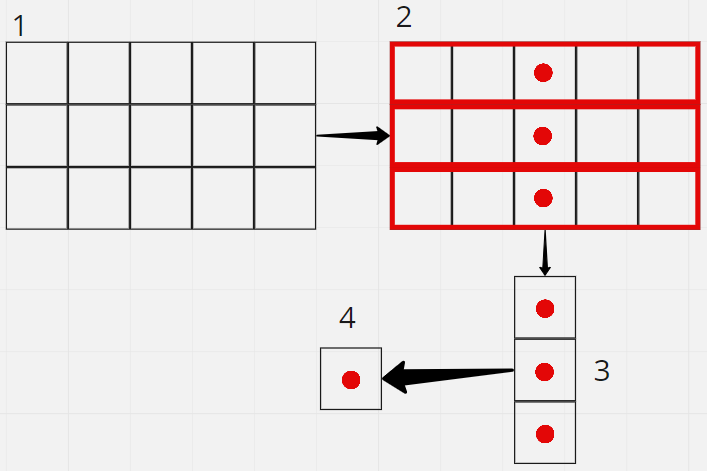
\includegraphics[width=8cm]{ejemplo.png}
	\centering
	\caption{Ejemplo}
	\label{fig:figura 1}
	\end{figure}
	
	\begin{figure}[h]
	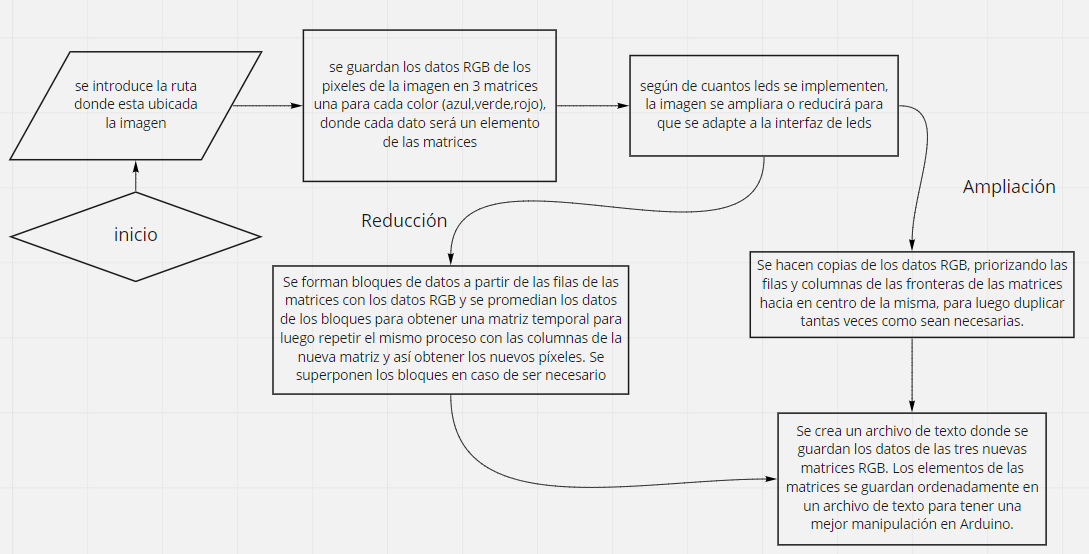
\includegraphics[width=12cm]{algoritmo.png}
	\centering
	\caption{Esquema de tareas}
	\label{fig:figura 2}
	\end{figure}
	
	\section{Consideraciones a tomar en cuenta}
	Luego de una discusión se propusieron las siguientes consideraciones a tener en cuente a la hora de realizar la implementación
	\begin{itemize}
	    \item La reducida capacidad de memoria de la tarjeta Arduino.
	    \item dependiendo de la clase de leds a implementar aumentará o disminuirá la complejidad de código. 
	    \item el segmento de código creado en Qt debe ser adaptado para el entorno Arduino.
	\end{itemize}
	\begin{figure}[h]
	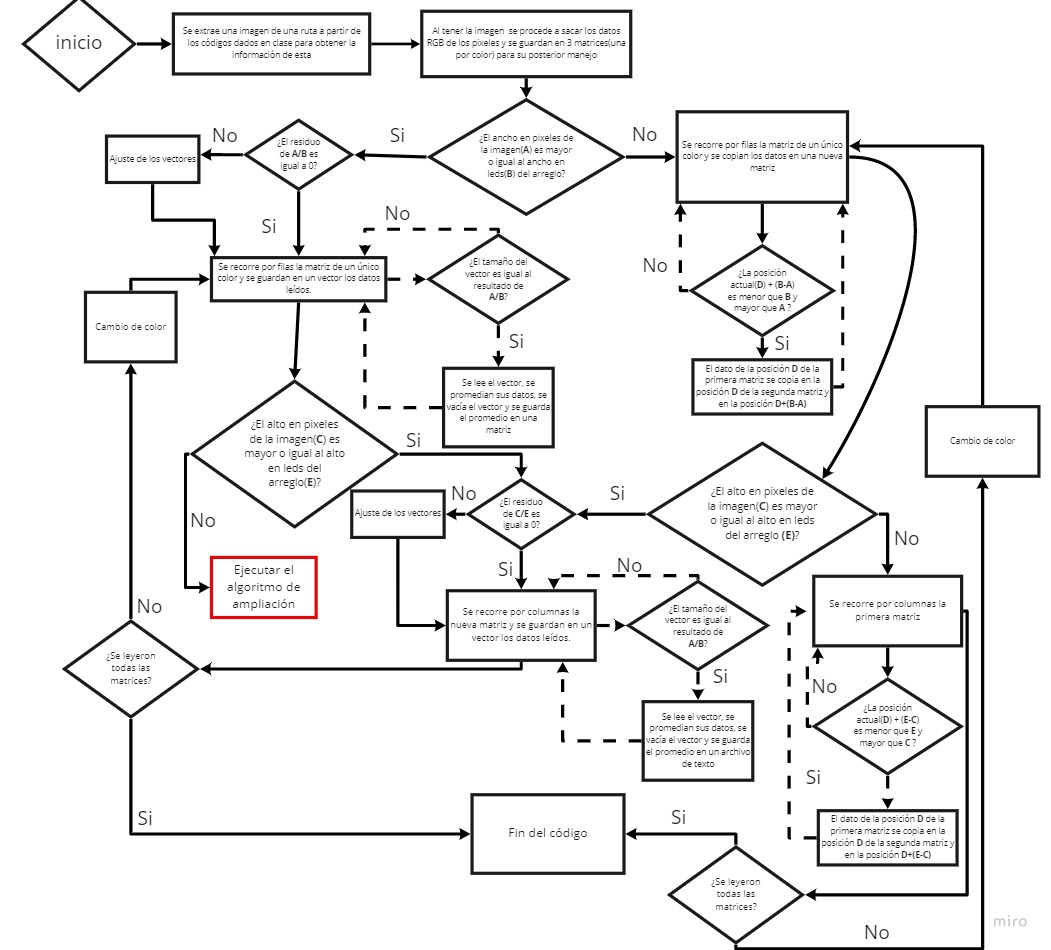
\includegraphics[width=12cm]{circuitando (7).jpg}
	\centering
	\caption{Algoritmo}
	\label{fig:figura 3}
	\end{figure}
	
\end{document}
